%%% Copyright (C) 2018 Vincent Goulet
%%%
%%% Ce fichier fait partie du projet
%%% «Rédaction avec LaTeX»
%%% http://github.com/vigou3/formation-latex-ul
%%%
%%% Cette création est mise à disposition selon le contrat
%%% Attribution-Partage dans les mêmes conditions 4.0
%%% International de Creative Commons.
%%% http://creativecommons.org/licenses/by-sa/4.0/

\begingroup

\TPGrid{3}{36}
\textblockorigin{0mm}{0mm}
\setlength{\parindent}{0mm}
\setlength{\banderougewidth}{2\TPHorizModule}
\setlength{\banderougeheight}{\TPVertModule}
\setlength{\bandeorwidth}{\TPHorizModule}
\setlength{\bandeorheight}{\banderougeheight}
\setlength{\imageheight}{29\TPVertModule}
\setlength{\imagewidth}{3\TPHorizModule}
\setlength{\logoheight}{3.5\TPVertModule}
\setlength{\gapwidth}{0.75pt}
\addtolength{\bandeorwidth}{-\gapwidth}
\addtolength{\imageheight}{-\gapwidth}

\def\titlefmt{%
  \titles\bfseries\fontsize{24}{24}\selectfont%
  Rédaction avec\par
  \rmfamily\mdseries\fontsize{22.5}{22.5}\selectfont%
  \raisebox{5pt}{{\textbackslash}title}%
  \fontsize{40}{40}\selectfont%
  \{%
  \fontsize{35}{35}\selectfont%
  \LaTeX
  \fontsize{40}{40}\selectfont%
  \}}
\def\subtitlefmt{%
  \titles\bfseries\fontsize{11}{11}\selectfont%
  Premiers pas\par}
\def\authorfmt{%
  \titles\bfseries\fontsize{14}{14}\selectfont%
  Vincent Goulet\par}
\def\affiliation{%
  \titles\mdseries\fontsize{11}{12}\selectfont%
  Professeur titulaire \\
  École d'actuariat, Université Laval}
\def\edition{%
  \titles\mdseries\fontsize{11}{11}\selectfont%
  Édition {\titles\year}.\month}

%%%
%%% Page de titre
%%%

\begin{frame}[plain]
  %% bandeau identitaire
  \begin{textblock*}{125mm}[0,1](0mm,30\TPVertModule)
    \textcolor{rouge}{\rule{\banderougewidth}{\banderougeheight}}% % bande rouge
    \rule{\gapwidth}{0pt}%                                         % filet
    \textcolor{or}{\rule{\bandeorwidth}{\bandeorheight}}           % bande or
  \end{textblock*}

  %% logo UL
  \begin{textblock*}{\TPHorizModule}(2\TPHorizModule,31\TPVertModule)
    \rule{\gapwidth}{0pt}%                                     % filet
    
\includegraphics[height=\logoheight,keepaspectratio=true]{ul_p}
  \end{textblock*}

  %% image de fond
  \begin{textblock*}{125mm}(0mm,0mm)
    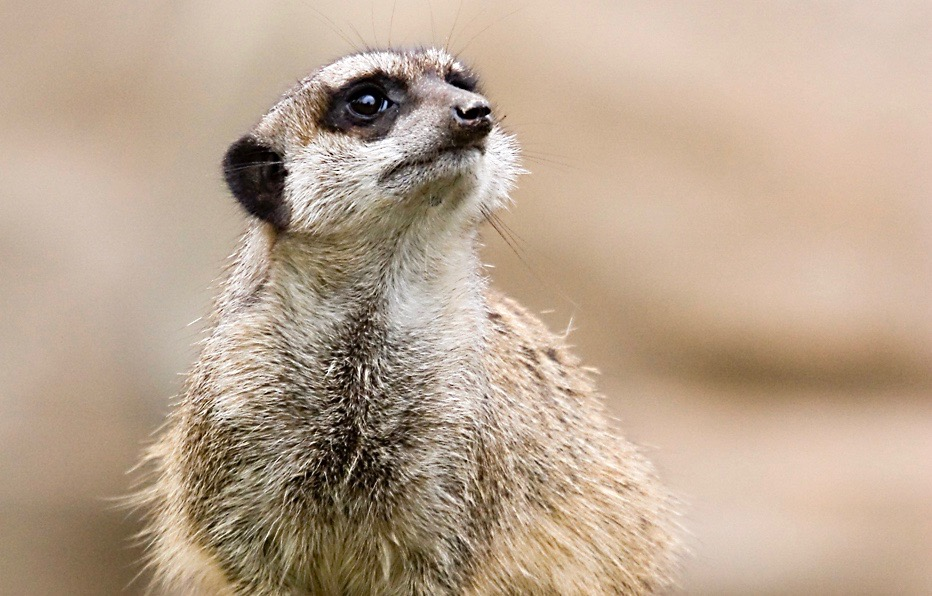
\includegraphics[width=\imagewidth,%
                     keepaspectratio=true]{Suricata-diapos.jpg}
  \end{textblock*}

  %% trame (titre)
  \begin{textblock*}{2\TPHorizModule}(0mm,14\TPVertModule)
    \pgfsetfillopacity{0.5}
    \textcolor{white}{\rule{\linewidth}{10\TPVertModule}}
    \pgfsetfillopacity{1}
  \end{textblock*}

  %% titre
  \begin{textblock*}{1.6\TPHorizModule}(0.4\TPHorizModule,15.2\TPVertModule)
    \titlefmt
  \end{textblock*}

  %% trame (premiers pas)
  \begin{textblock*}{\TPHorizModule}(2\TPHorizModule,24\TPVertModule)
    \pgfsetfillopacity{0.5}
    \textcolor{white}{\rule{\linewidth}{2\TPVertModule}}
    \pgfsetfillopacity{1}
  \end{textblock*}

  %% sous-titre (premiers pas)
  \begin{textblock*}{0.8\TPHorizModule}(2.1\TPHorizModule,24.5\TPVertModule)
    \subtitlefmt
  \end{textblock*}
\end{frame}

%%%
%%% Page frontispice
%%%

\begin{frame}[plain]
  \begin{textblock*}{1.6\TPHorizModule}(0.4\TPHorizModule,5\TPVertModule)
    \authorfmt
  \end{textblock*}

  \begin{textblock*}{1.6\TPHorizModule}(0.4\TPHorizModule,7\TPVertModule)
    \affiliation
  \end{textblock*}

  \begin{textblock*}{1.6\TPHorizModule}(0.4\TPHorizModule,15.2\TPVertModule)
    \titlefmt
  \end{textblock*}

  \begin{textblock*}{1.6\TPHorizModule}(0.4\TPHorizModule,30\TPVertModule)
    \edition
  \end{textblock*}
\end{frame}
\endgroup

%%% Local Variables:
%%% TeX-master: "formation-latex-ul-diapos"
%%% TeX-engine: xetex
%%% coding: utf-8
%%% End:
